%
% herleitung.tex -- Bild zum Thema Optische Fouriertransformation <opt>
%
% (c) 2023 Marco Niederberger, Yanick Schoch; OST Ostschweizer Fachhochschule
%

\documentclass[tikz]{standalone}
% \usepackage{amsmath}
% \usepackage{txfonts}
% \usepackage{pgfplots}

% \pgfplotsset{compat=1.16}
\def\skala{1}

%
% opt_common.tex -- Commands and color definition for the paper <opt>
%
% (c) 2023 Marco Niederberger, Yanick Schoch; OST Ostschweizer Fachhochschule
%

%%% NEW COMMANDS %%%

% Lense (x, height, curvature)
\newcommand{\lense}[3]{
    \def\curvature{0.2}
    \path[fill=glass, draw=black, line width = 0.6, opacity=0.8] (#1,-#2) .. controls (#1 - #3,0) .. (#1,#2) .. controls (#1 + #3,0) .. (#1,-#2);
}

% Dimension arrow (xStart, xEnd, yHeight, text)
\newcommand{\optMeasurement}[4]{%
    \draw[<->] (#1, #3)--(#2, #3) node[above,midway] {#4};
}

% Annotated point
\newcommand{\point}[3]{
    \draw[fill=black] (#1) circle (1pt) node[#3] {#2};
}

%%% COLORS %%%

% Define Color
\definecolor{glass}{cmyk}{0.2,0,0,0}
\colorlet{optBlue}{blue!70!black}
\colorlet{optRed}{red!90!black}

%%% STYLES %%%

% Laser rays
\tikzset{red ray/.style = {optRed, line width = 0.6}}
\tikzset{ray arrow/.style = {red ray, postaction=decorate,decoration={markings,mark=at position 0.52 with \arrow{stealth}}}}


% \usetikzlibrary{arrows,intersections,math}
\usetikzlibrary{decorations.markings, } %calc


\begin{document}

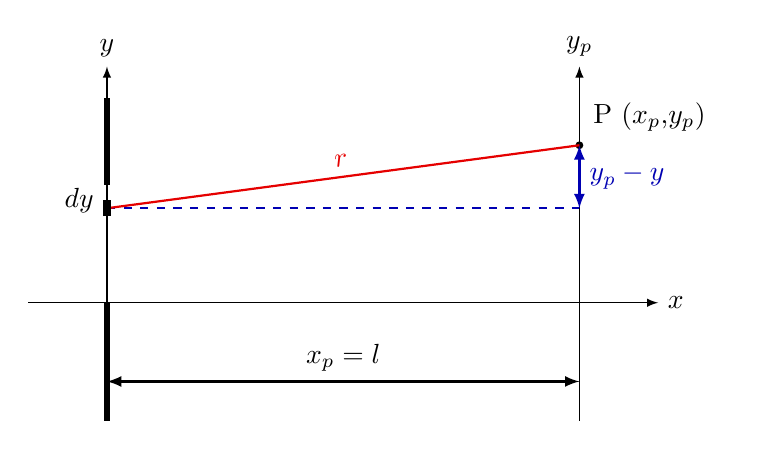
\begin{tikzpicture}[>=latex,thick,scale=\skala]
    % \draw[help lines, color=gray!30, dashed] (-10,-5) grid (10,5);

    \draw[draw=none] (-1,0)--(8,0);
    % Define points
    \coordinate (P) at (6,2);
    \coordinate (E) at (0,1.2);

    % x and y axis
    \draw[->, thin] (-1,0)--(7,0) node[right]{$x$};
    \draw[->, thin] (6,-1.5)--(6,3) node[above]{$y_p$};
    \draw[->, thin] (0,-1.5)--(0,3) node[above]{$y$};

    % Aperture
    \draw[line width=2, black] (0, 1.5)--(0, 2.6);
    \draw[line width=2, black] (0, 0)--(0, -1.5);
    
    \node[label={45:{P ($x_p$,$y_p$)}}, circle, fill, inner sep=1pt] at (P) {};
    
    
    \draw[optBlue, dashed] (E) -- (6,1.2);
    \draw[optBlue, <->] (P) -- (6,1.2) node[midway, right]{$y_p - y$};
    
    \draw[optRed] (E) -- (P) node[midway, sloped, above]{$r$};

    \draw[line width=3pt] (0,1.1)--(0,1.3) node[left]{$dy$};

    \optMeasurement{0}{6}{-1}{$x_p = l$}

\end{tikzpicture}
\end{document}

